\KOMAoptions{paper=A3}
\recalctypearea
\subsection{Farey Sequence}{\label{pp:fareysequence}}
Farey sequence has all rational numbers in range $[0/1\ \text{to}\ 1/1]$ sorted \emph{in increasing order} such that the denominators are less than or equal to $n$ and all numbers are in \emph{reduced forms} i.e., 2/4 does not belong to this sequence as it can be reduced to 1/2.\\
For example, $n=4$, the possible rational numbers in increasing order are $\ 0/1,\ 1/4,\ 1/3,\ 1/2,\ 2/3,\ 3/4,\ 1/1$.
\vspace{-1em}
\subsubsection*{Stern-Brocot Tree}
\vspace{-0.7em}
To generate the Farey Sequence, we have to first look at the {Stern-Brocot Tree} shown in \ref{fig:sternbrocottree}.
\begin{figure}[H]
	\centering
	\scalebox{1}[0.8]{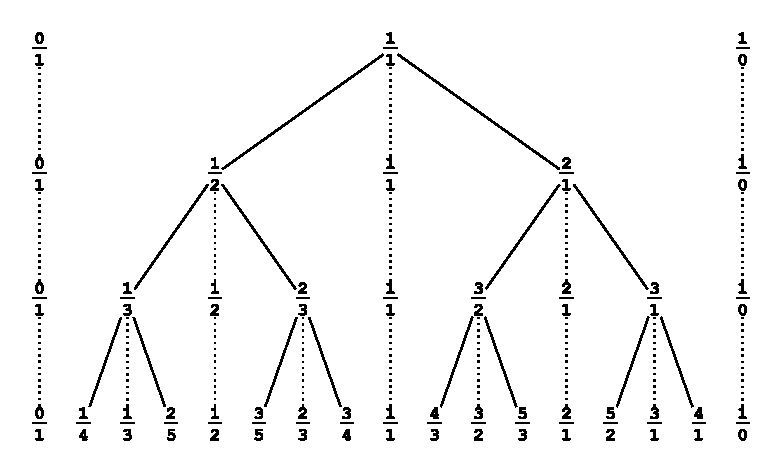
\includegraphics[width=0.6\linewidth]{Stern-Brocot Tree.pdf}}
	\caption{The Stern-Brocot Tree for Level $1-4$ (\href{https://commons.wikimedia.org/wiki/File:SternBrocotTree.svg}{Image} by \href{https://commons.wikimedia.org/wiki/User:Aaron_Rotenberg}{Aaron Rotenberg} licensed under \href{https://creativecommons.org/licenses/by-sa/3.0/}{CC BY-SA 3.0})}
	\label{fig:sternbrocottree}
\end{figure}
In this tree, a child is given by the \href{https://en.wikipedia.org/wiki/Mediant_(mathematics)}{mediant} of their parents; i.e, for child of parents $\mfrac{a}{c}$ and $\mfrac{b}{d}$ is $\mfrac{a+b}{c+d}$.

Some examples for parent, child are as follows -- $\left(\mfrac{0}{1}, \mfrac{1}{1} \rightarrow \mfrac{1}{2}\right)$, $\left(\mfrac{1}{1}, \mfrac{1}{0} \rightarrow \mfrac{2}{1}\right)$, $\left(\mfrac{0}{1}, \mfrac{1}{2} \rightarrow \mfrac{1}{3}\right)$, $\left(\mfrac{1}{2}, \mfrac{1}{1} \rightarrow \mfrac{2}{3}\right)$, $\left(\mfrac{1}{1}, \mfrac{2}{1} \rightarrow \mfrac{3}{2}\right)$, $\left(\mfrac{2}{1}, \mfrac{1}{0} \rightarrow \mfrac{3}{1}\right)$,

Notice that the farey sequence for corresponding $n$ is the subset of vertices of this tree calculated upto level $n$.

Also, for every fraction $\mfrac{p}{q}$ in the farey sequence draw a circle with centre at $\left(\mfrac{p}{q}, \mfrac{1}{2q^2}\right)$ and radius $\left(\mfrac{1}{2q^2}\right)$. You may need to do some scaling to get a proper figure.

\textbf{Problem Statement:}\\
Generate the Farey Sequence for corresponding $n$ using ideas from the Stern-Brocot Tree or otherwise and draw the circles.
\begin{hint}
	Recursion!
\end{hint}
\begin{testcasesMore}
	{$n$ \hfill(a single integer)}
	{Corresponding numbers in farey sequence in $p/q$ format with the circles.}
	{$1\leq n\leq 30$ \hfill(an integer)}
	{7}
	{0/1 1/7 1/6 1/5 1/4 2/7 1/3 2/5 3/7 1/2 4/7 3/5 2/3 5/7 3/4 4/5 5/6 6/7 1/1}
	% {0/1 1/1\\0/1 1/2 1/1\\0/1 1/3 1/2 2/3 1/1\\0/1 1/4 1/3 1/2 2/3 3/4 1/1\\0/1 1/5 1/4 1/3 2/5 1/2 3/5 2/3 3/4 4/5 1/1\\0/1 1/6 1/5 1/4 1/3 2/5 1/2 3/5 2/3 3/4 4/5 5/6 1/1\\0/1 1/7 1/6 1/5 1/4 2/7 1/3 2/5 3/7 1/2 4/7 3/5 2/3 5/7 3/4 4/5 5/6 6/7 1/1\\0/1 1/8 1/7 1/6 1/5 1/4 2/7 1/3 3/8 2/5 3/7 1/2 4/7 3/5 5/8 2/3 5/7 3/4 4/5 5/6 6/7 7/8 1/1\\0/1 1/13 1/12 1/11 1/10 1/9 1/8 1/7 2/13 1/6 2/11 1/5 2/9 3/13 1/4 3/11 2/7 3/10 4/13 1/3 4/11 3/8 5/13 2/5 5/12 3/7 4/9 5/11 6/13 1/2 7/13 6/11 5/9 4/7 7/12 3/5 8/13 5/8 7/11 2/3 9/13 7/10 5/7 8/11 3/4 10/13 7/9 4/5 9/11 5/6 11/13 6/7 7/8 8/9 9/10 10/11 11/12 12/13 1/1\\0/1 1/21 1/20 1/19 1/18 1/17 1/16 1/15 1/14 1/13 1/12 1/11 2/21 1/10 2/19 1/9 2/17 1/8 2/15 1/7 3/20 2/13 3/19 1/6 3/17 2/11 3/16 4/21 1/5 4/19 3/14 2/9 3/13 4/17 5/21 1/4 5/19 4/15 3/11 5/18 2/7 5/17 3/10 4/13 5/16 6/19 1/3 7/20 6/17 5/14 4/11 7/19 3/8 8/21 5/13 7/18 2/5 7/17 5/12 8/19 3/7 7/16 4/9 9/20 5/11 6/13 7/15 8/17 9/19 10/21 1/2 11/21 10/19 9/17 8/15 7/13 6/11 11/20 5/9 9/16 4/7 11/19 7/12 10/17 3/5 11/18 8/13 13/21 5/8 12/19 7/11 9/14 11/17 13/20 2/3 13/19 11/16 9/13 7/10 12/17 5/7 13/18 8/11 11/15 14/19 3/4 16/21 13/17 10/13 7/9 11/14 15/19 4/5 17/21 13/16 9/11 14/17 5/6 16/19 11/13 17/20 6/7 13/15 7/8 15/17 8/9 17/19 9/10 19/21 10/11 11/12 12/13 13/14 14/15 15/16 16/17 17/18 18/19 19/20 20/21 1/1}
	{https://github.com/paramrathour/CS-101/tree/main/Test Cases/Farey Sequence/Input}
	{https://github.com/paramrathour/CS-101/tree/main/Test Cases/Farey Sequence/Output}
	{https://github.com/paramrathour/CS-101/tree/main/Starter Codes/Farey Sequence.cpp}
\end{testcasesMore}
\textbf{The output circles (Ford Circles)}
\begin{figure}[H]
	\centering
	\begin{subfigure}{0.3\linewidth}
		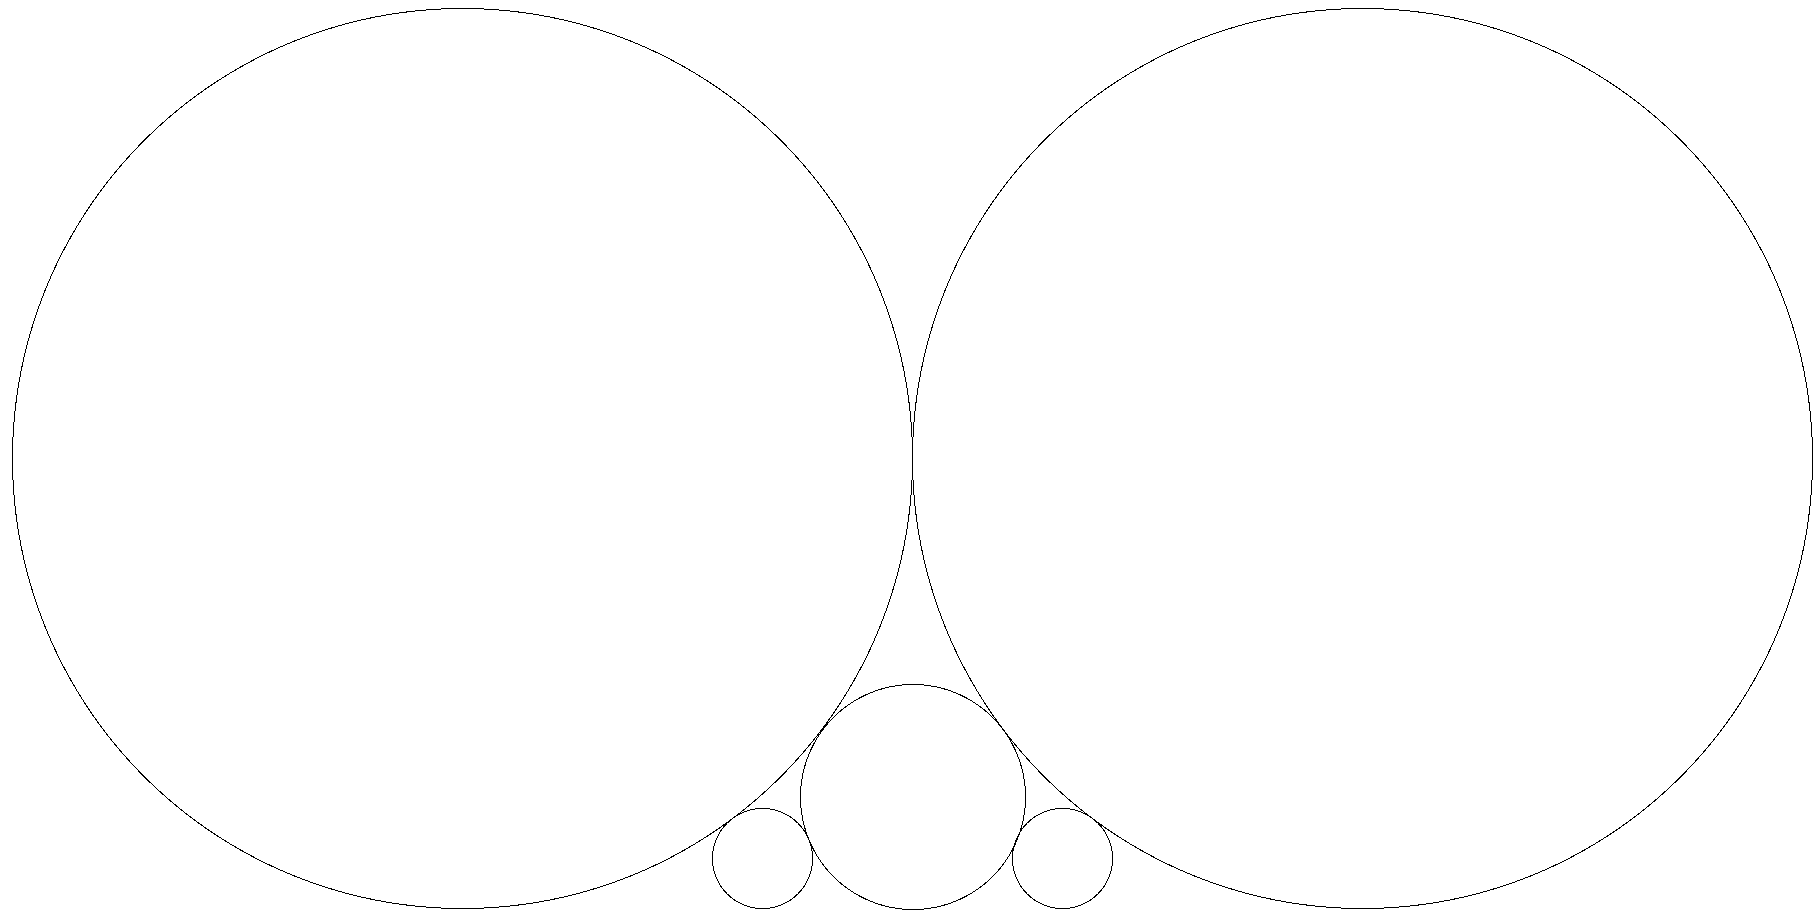
\includegraphics[width = \linewidth]{Farey Sequence/3.png}
		\caption{$n=3$}
	\end{subfigure}
	\begin{subfigure}{0.3\linewidth}
		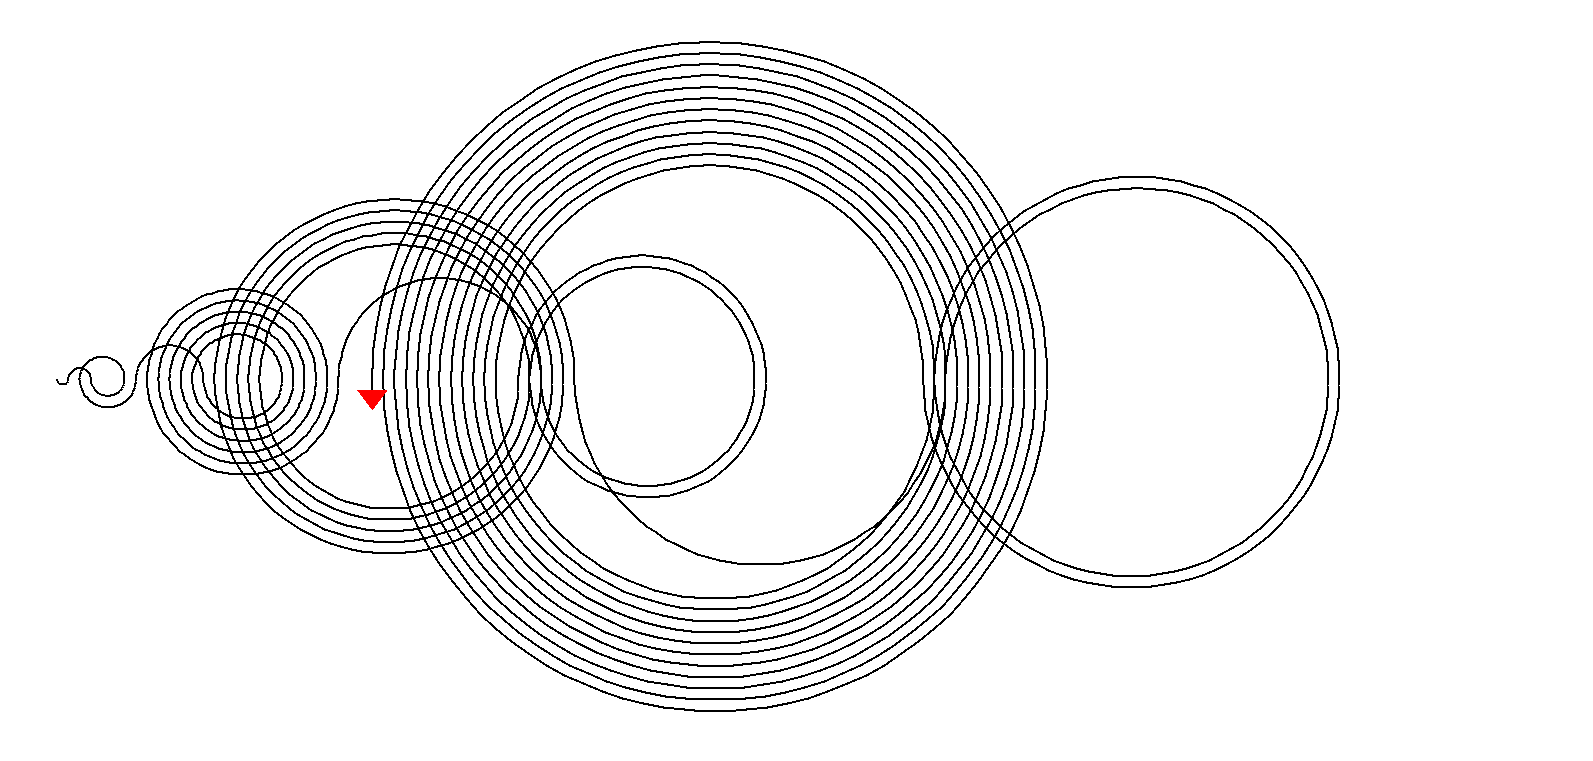
\includegraphics[width = \linewidth]{Farey Sequence/7.png}
		\caption{$n=7$}
	\end{subfigure}
	\begin{subfigure}{0.3\linewidth}
		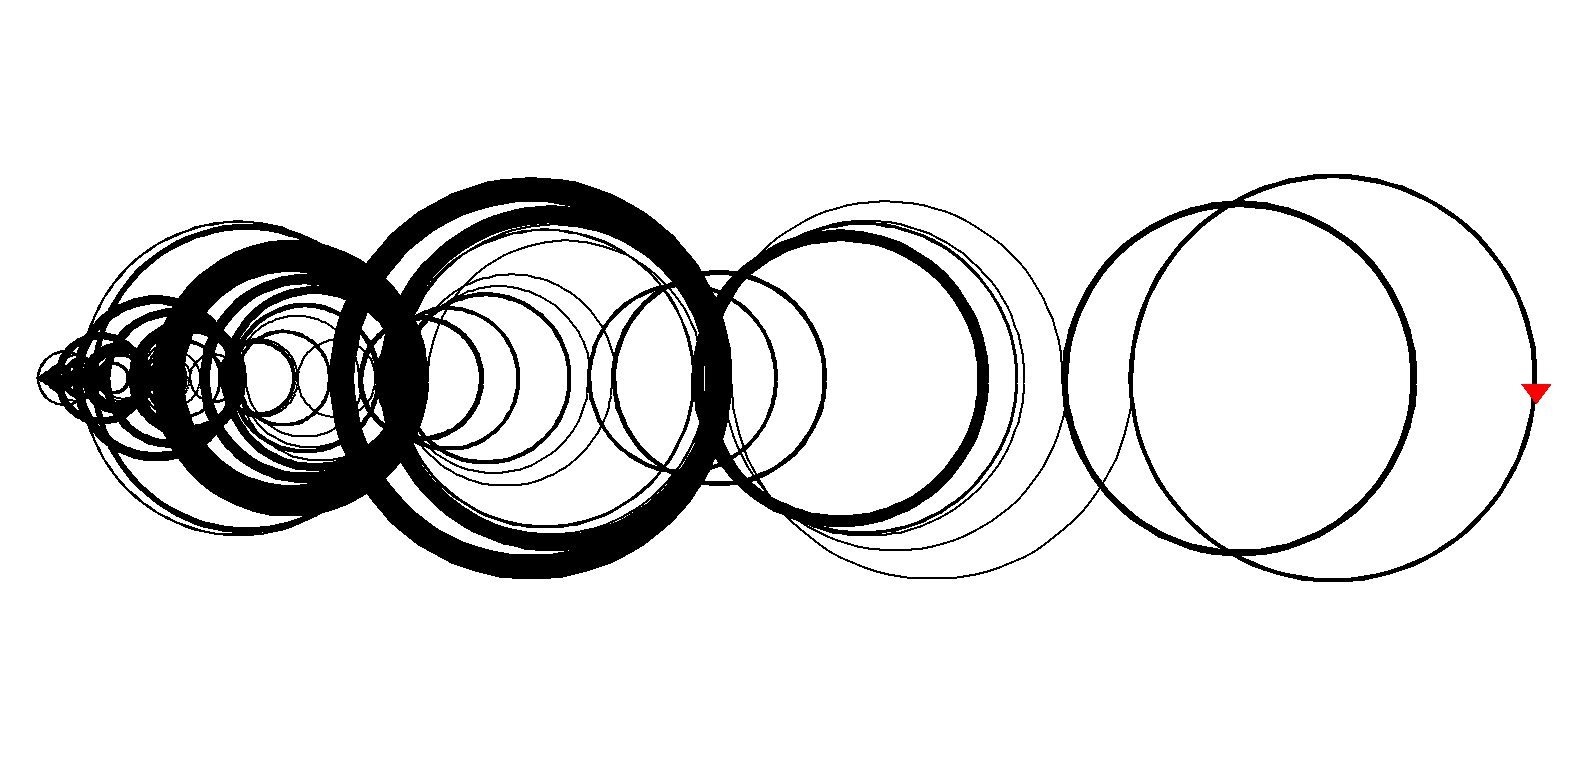
\includegraphics[width = \linewidth]{Farey Sequence/10.png}
		\caption{$n=10$}
	\end{subfigure}
	\caption{Output Ford Circles for few $n$}
\end{figure}
\begin{noteI}
	If the outputs take a long time then how can you make it faster?. Also, try calculating terms mathematically to get the fastest way!
\end{noteI}
\begin{funvideo}
\href{https://youtu.be/DpwUVExX27E}{Infinite Fractions -- Numberphile}\\
\href{https://youtu.be/0hlvhQZIOQw}{Funny Fractions and Ford Circles -- Numberphile}
\end{funvideo}
\KOMAoptions{paper=A4}
\recalctypearea